%%%%%%%%%%%%%%%%%%%%%%%%%%%%%%%%%%%%%%%%%
% Short Sectioned Assignment
% LaTeX Template
% Version 1.0 (5/5/12)
%
% This template has been downloaded from:
% http://www.LaTeXTemplates.com
%
% Original author:
% Frits Wenneker (http://www.howtotex.com)
%
% License:
% CC BY-NC-SA 3.0 (http://creativecommons.org/licenses/by-nc-sa/3.0/)
%
%%%%%%%%%%%%%%%%%%%%%%%%%%%%%%%%%%%%%%%%%

%----------------------------------------------------------------------------------------
%	PACKAGES AND OTHER DOCUMENT CONFIGURATIONS
%----------------------------------------------------------------------------------------

\documentclass[paper=a4, fontsize=11pt]{scrartcl} % A4 paper and 11pt font size

\usepackage[T1]{fontenc} % Use 8-bit encoding that has 256 glyphs
%\usepackage{fourier} % Use the Adobe Utopia font for the document - comment this line to return to the LaTeX default
\usepackage[english]{babel} % English language/hyphenation
\usepackage{amsmath,amsfonts,amsthm,amssymb} % Math packages

\usepackage{sectsty} % Allows customizing section commands
%\allsectionsfont{\centering \normalfont\scshape} % Make all sections centered, the default font and small caps
\allsectionsfont{\centering}

\usepackage{fancyhdr} % Custom headers and footers
\pagestyle{fancyplain} % Makes all pages in the document conform to the custom headers and footers
\fancyhead{} % No page header - if you want one, create it in the same way as the footers below
\fancyfoot[L]{} % Empty left footer
\fancyfoot[C]{} % Empty center footer
\fancyfoot[R]{\thepage} % Page numbering for right footer
\renewcommand{\headrulewidth}{0pt} % Remove header underlines
\renewcommand{\footrulewidth}{0pt} % Remove footer underlines
\setlength{\headheight}{13.6pt} % Customize the height of the header

%\numberwithin{equation}{section} % Number equations within sections (i.e. 1.1, 1.2, 2.1, 2.2 instead of 1, 2, 3, 4)
%\numberwithin{figure}{section} % Number figures within sections (i.e. 1.1, 1.2, 2.1, 2.2 instead of 1, 2, 3, 4)
%\numberwithin{table}{section} % Number tables within sections (i.e. 1.1, 1.2, 2.1, 2.2 instead of 1, 2, 3, 4)

\setlength\parindent{0pt} % Removes all indentation from paragraphs - comment this line for an assignment with lots of text

\usepackage{caption}

\usepackage{algorithm}
\usepackage[noend]{algorithmic}

%\floatname{algorithm}{Procedure}
\renewcommand{\algorithmicrequire}{\textbf{Input:}}
\renewcommand{\algorithmicensure}{\textbf{Output:}}

\newtheorem{mydef}{Definition}
\theoremstyle{plain}
\newtheorem{lemma}{Lemma}


\usepackage{graphicx}
\graphicspath{{../images/}}



%----------------------------------------------------------------------------------------
%	TITLE SECTION
%----------------------------------------------------------------------------------------

\newcommand{\horrule}[1]{\rule{\linewidth}{#1}} % Create horizontal rule command with 1 argument of height

\title{	
\normalfont \normalsize 
\textsc{UPC - Discrete and algorithmic geometry} \\ [25pt] % Your university, school and/or department name(s)
\horrule{0.5pt} \\[0.4cm] % Thin top horizontal rule
\huge Problem sheet 2  \\ % The assignment title
\horrule{2pt} \\[0.5cm] % Thick bottom horizontal rule
}

\author{Simon Van den Eynde \\ Petar Hlad Colic} % Your name

\date{\normalsize\today} % Today's date or a custom date

\begin{document}

\maketitle % Print the title

\section{Nonrational Pentagon}
Given the incidences we have given, we should show that the inner pentagon is regular, then we can use http://mathworld.wolfram.com/Pentagon.html to show the construction cannot be realised with rational coordinates.

\section{6.9: enumerate 4-polytopes with 7 vertices}

To enumerate all 4-polytopes with 7-vertices, we started considering only these with a Gale diagram without special points and without coinciding points. For finding these polytopes we wrote an algorithm.\\

We start considering all possible Gale diagrams, this is a list of $7$ $+$'s and $-$'s. First we filtered all diagrams that couldn't come from a polytope. For doing this, we used Theorem 6.19 in Ziegler, which says that a Gale diagram relates to a polytope $\iff$ every cocircuit has at least $2$ positive elements. This we can check by, for every index, checking the plusses after the index and the minuses before the index and making sure they sum up to at least $2$.\\

Then we filtered out the isomorphism, by creating the graph of the facet structure and check wether these are isomorphic. For checking this we used a graphlibrary.\\

Finally we find $5$ non-isomorphic Gale diagrams:
\[[0, 0, 1, 1, 0, 0, 1],
 [0, 0, 1, 0, 1, 0, 1],
 [0, 1, 0, 1, 0, 0, 1],
 [0, 1, 0, 0, 1, 0, 1],
 [1, 0, 1, 0, 1, 0, 1]\]
 


\section{6.15: 2 different 2-neighborly 4-polytopes}
We can easily check that both polytopes are $2$-neighborly, since removing any two points from the Gale diagram and then taking the convex hull of the positive and of the negative points, we find that these intersect. Thus the two removed points form an edge. I checked this manually, but I haven't written this down, using symmetries you should have to check around $30$ intersections.\\

If we write down all facets from the first Gale diagram, using the fact that circuits define cofacets. And also from $C_4(8)$, using Gale's evenness criterium, we find that exactly the same structure appears (even the naming is already correct). If we write down the facets from the second Gale diagram, we note there are differences, since their are different convex hulls (we also get the intersection of a triangle and a point).\\

To make sure that the second graph differs from the first, we used the sagemath graph library (a python-based mathematical computer language) to compare the graphs of the facetstructure. I generated images for both graphs: see figure~\ref{fig:1} and figure~\ref{fig:2}. Using the isomorphism-function of the graph library, we find that both graphs are different.

\begin{figure}[htbp] %  figure placement: here, top, bottom, or page
   \centering
   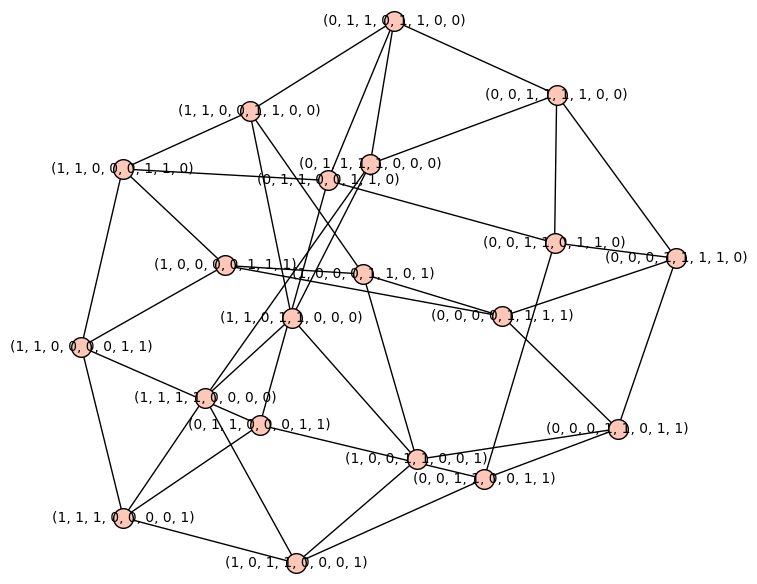
\includegraphics[width=\textwidth]{C4(8)} 
   \caption{The facet-graph of C4(8). Vertices are facets, and edges represent ridges between two facets.}
   \label{fig:1}
\end{figure}

\begin{figure}[htbp] %  figure placement: here, top, bottom, or page
   \centering
   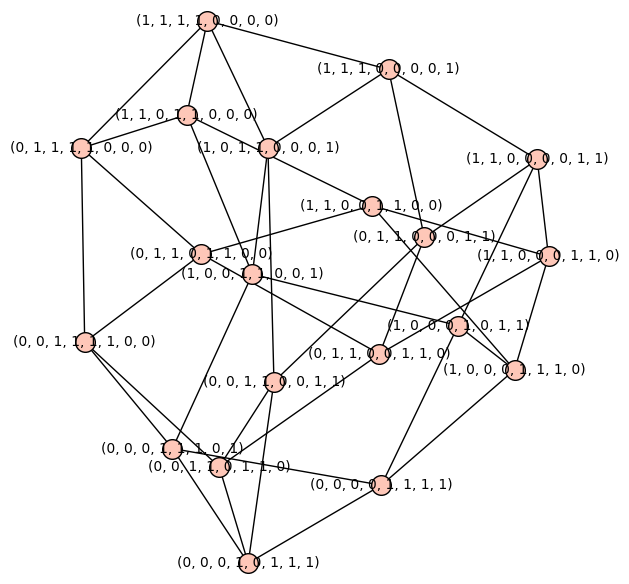
\includegraphics[width=\textwidth]{secondGale} 
   \caption{The facet-graph of the second Gale diagram. Vertices are facets, and edges represent ridges between two facets.}
   \label{fig:2}
\end{figure}



 
\section{6.17: analyse gale diagram}
We can find the facets by finding circuits in the Gale diagram. For example the convex hull of $\{1\}$ and $\{4\}$ intersect, so 14 is a cofacet and 235678 a facet of $P$. To check that this is an octahedron, we lift $14$ to infinity, and put the rest on one line, we get as Gale diagram a line with following points: $2^-,3^+6^+,7^-8^-,5^+$. If we look at the facet structure of the polytope with this Gale diagram, we see the polytope is $4$-regular, has $2$ vertices $2$ and $5$ which are neighbours of $3,6,7,8$ and that $3\sim 78,6\sim 78, 7\not\sim 8$ and $3\not\sim 6$. This is exactly the incidence structure of an octahedron.

For example we also find the cofacet 3457 which results in a facet 1268. Because this facet has $4$ vertices in dimension $3$, it is a simplex. We find some other simplices: $1267,3457,3458$.

We also find facets: $14568,14567,12347,12348$. To be a square pyramid they need a special point (a zero-point which is non-plus and non-negative), but I don't know how to get one.\\

If we have the same circuits, we have the same intersections in our Gale diagram so both 7 and 8 should lie on the line 23 and on the line 56, since these lines are different and the intersection is a single point, they must lie on the same point.\\

XXX Then 2356 lie in the same plane.\\

Since 2356 must be coplanar, we cannot chose all of them freely and the octahedral facet cannot be prescribed.\\

XXX The oriented matroid is not rigid, I don't know yet.

\end{document}











